\section{Methodology}

\subsection{Framework Overview}

In this section, we introduce {\method}, a novel agent framework designed for \textit{Productivity Tasks} $\mathcal{T}_{prod}$ without finetuning LLMs.
To enable this test-time learning paradigm, {\method} continuously interacts with a comprehensive environment $\mathcal{E}$ that comprises multiple software and platforms, such as chat application, code editors, and web browsers. Within this environment, the agent executes actions $a_t$ via a predefined basic toolset $\mathcal{A}_{tool}$. The architecture of {\method} includes three core components designed to support this interactive learning loop: a Memory Module $\mathcal{M}$ (Sec.~\ref{sec:memory}), a Planning-Execution (PE) Agent (Sec.~\ref{sec:pe agent}), and a Reflect Agent (Sec.~\ref{sec:reflect agent}). The Memory Module is further decomposed into three functionally distinct components: Strategic Memory~$\mathcal{M}_{strat}$, Procedural Memory~$\mathcal{M}_{proc}$, and Tool Memory~$\mathcal{M}_{tool}$.


As illustrated in Figure~\ref{fig:pipeline}, the operational mechanism of our framework is a ``Plan-Execute-Reflect-Memorize'' iterative loop. The system begins by initializing and loading the Memory Module ($\mathcal{M}$). When a new task ($\tau \in \mathcal{T}_{prod}$) is received, the process unfolds as follows.
\textbf{1) Plan and Execute:}
The PE Agent initiates the process by performing a preliminary analysis of the task, decomposing it into an ordered queue of sub-tasks. For each sub-task, the PE Agent first queries the Procedural Memory to retrieve guidance from relevant prior knowledge. It then executes a sequence of actions in the interactive environment $\mathcal{E}$ using a deliberately minimal toolset. Each fundamental interaction step involves the agent receiving an observation $o_t$ and, based on its history $h_t = (o_{1:t}, a_{1:t-1})$, selecting an action via its policy $a_t \sim \pi_{\text{test}}(a_t \mid h_t)$. This design compels the agent to learn how to compose primitive tool actions into complex workflows required to accomplish the sub-tasks. The execution phase for a given sub-task concludes once the PE Agent deems its attempt complete.
\textbf{2)~Reflect and Memorize:}
After each sub-task attempt, the Reflect Agent conducts an autonomous assessment based on its environmental observations and the PE Agent's sub-task execution trajectory $h_{k:t} = (o_{k:t}, a_{k:t-1})$, requiring no human intervention. If the sub-task is successful, the Reflect Agent distills the trajectory into new \textit{Procedural Memory}. Otherwise, it generates a diagnostic analysis of the failure and instructs the PE Agent to replan and re-execute. The PE Agent adaptively refreshes its overall task plan after each assessment, continuing this core loop until the entire task is complete.
\textbf{3) Post-Task Distill:}
Upon completing the overall task, a comprehensive task analysis is conducted on the full execution trajectory. From this analysis, the Reflect Agent distills higher-level \textit{Strategic} and \textit{Tool Memories}, capturing broader insights and effective guidelines. Ultimately, all memory types—Procedural, Strategic, and Tool—are uniformly maintained within $\mathcal{M}$, ensuring the effective retention and future applicability of all acquired knowledge.

\begin{figure}[tbp]
    \begin{center}
    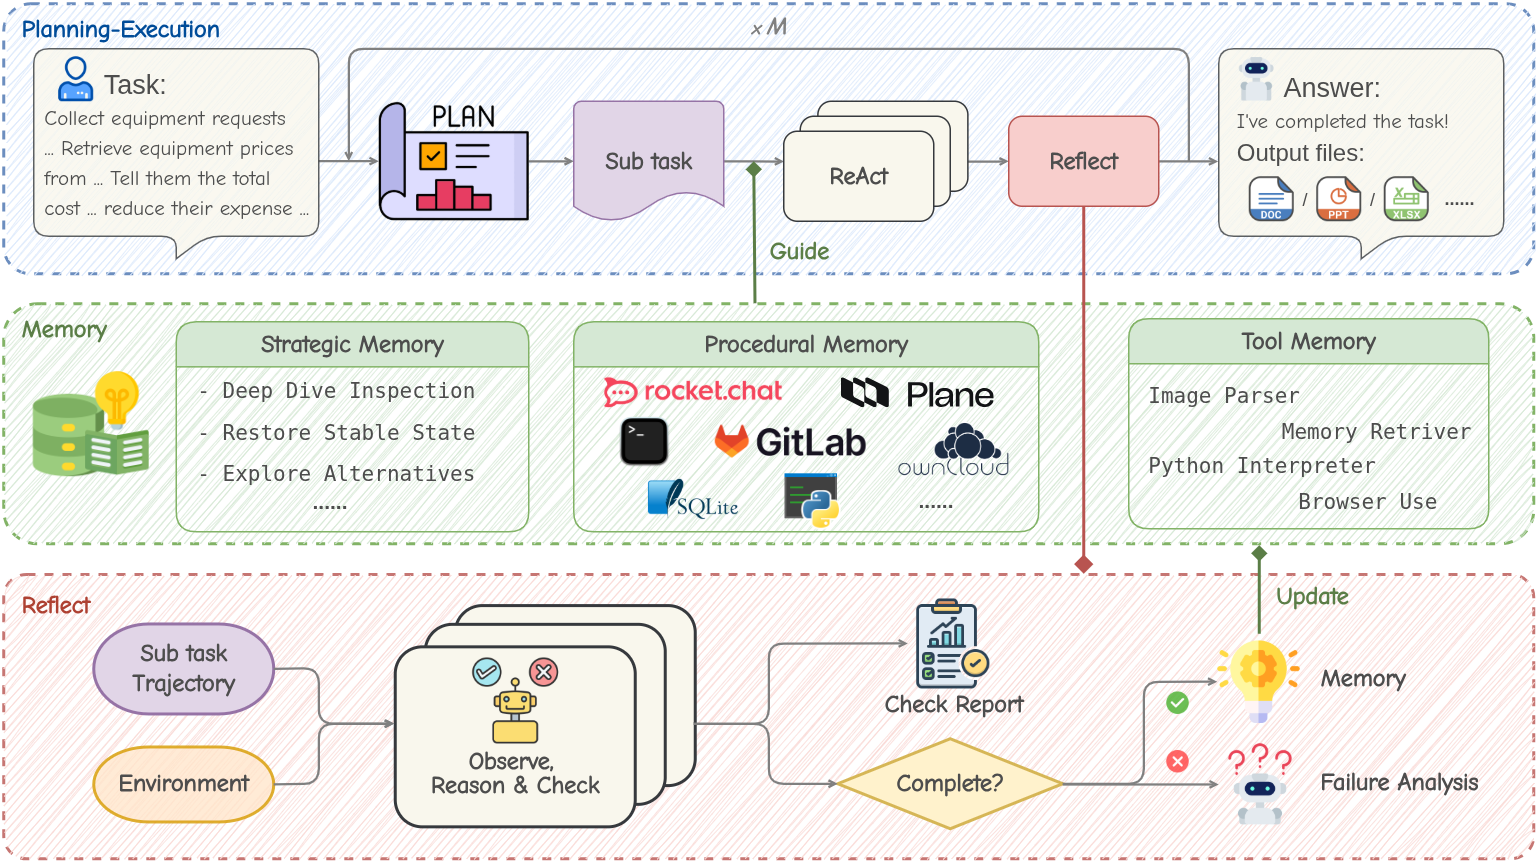
\includegraphics[width=0.95\linewidth]{figures/pipeline.png}
    
    % \vspace{-10pt}
    \end{center}
   \caption{The {\method} framework adopts a ``Plan-Execute-Reflect-Memorize'' loop. The \textbf{Planning-Execution(PE) Agent} decomposes task and performs actions within an interactive environment, while the \textbf{Reflect Agent} abstracts successful attempts into Procedural Memory. After task completion, the Reflection Agent further synthesizes this knowledge into the Strategic and Tool Memory.}
     \label{fig:pipeline}
    \vspace{-10pt}
\end{figure}


\subsection{Memory Module}
\label{sec:memory}


The Memory Module $\mathcal{M}$ is the key component enabling our {\method} to learn on the job. 
{Given the high expense of fine-tuning and our goal of maximizing the utility of closed-source LLMs, we refrain from fine-tuning the base LLM to maintain its native generalization capacity. Rather, we incrementally build up $\mathcal{M}$, allowing the agent’s performance $R(t)$ to improve over repeated trials on tasks $\tau \in \mathcal{T}_{prod}$.}
This module is a composite memory $\mathcal{M} = \{\mathcal{M}_{strat}, \mathcal{M}_{proc}, \mathcal{M}_{tool}\}$ comprising three distinct memory types, each optimized for a specific level of abstraction: Strategic Memory $\mathcal{M}_{strat}$ for macro-level behavioral paradigms, Procedural Memory $\mathcal{M}_{proc}$ for combinations of tool sequences, and Tool Memory $\mathcal{M}_{tool}$ for individual tool use. Each memory type operates with distinct mechanisms for its generation, updating, and application.

\textbf{Strategic Memory} ($\mathcal{M}_{strat}$) focuses on distilling lessons from dilemmas an agent encounters during task execution and their solutions, particularly from challenges that require multiple attempts to overcome. The Reflect Agent abstracts these ``problem-solution'' experiences into high-level guidance and formats them as $\textless \text{Dilemma}, \text{Strategy} \textgreater$ key-value pairs. Upon agent initialization, the entire $\mathcal{M}_{strat}$ is loaded into the system prompt to guide its global task execution strategy. To ensure efficiency and prevent context window bloat, this memory is updated, merged, and refined after each task, always maintaining a concise size. For specific examples, refer to \Cref{tab:strategic_memory} in the appendix.

\textbf{Procedural Memory} ($\mathcal{M}_{proc}$) archives the PE Agent's successful sub-task trajectories as a hierarchical knowledge base of Standard Operating Procedures (SOPs). This library is indexed first by application (e.g., related platforms or APIs), followed by a second-level SOP index that documents the key analyses, precaution, core parameters, and operational steps for each sub-task.
To balance efficiency and performance, the system employs a lightweight, proactive retrieval mechanism. Only the SOP index is loaded at startup to minimize overhead. When facing uncertainty, the agent utilizes a built-in tool to proactively query detailed SOPs for decision support, which closely mimics how human experts consult past cases. The memory system is refined through a two-stage process. First, immediately following a successful sub-task, the Reflect Agent dynamically adds the new SOP $p_{new}$ to $\mathcal{M}_{proc}$ for immediate reuse. Second, after the entire task is complete, the agent performs a higher-level, global refinement (e.g., deduplication, generalization) to continuously optimize the long-term quality and applicability of the knowledge base.
See \Cref{tab:procedural_memory} in the appendix for examples.

\textbf{Tool Memory} ($\mathcal{M}_{tool}$) functions as the agent's ``muscle memory'' for single tool usage, operating automatically without requiring proactive retrieval. This memory consists of two components, $\mathcal{M}_{tool} = \{D_{static}, I_{dynamic}\}$: A Static Description $D_{static}$, loaded into the system prompt at startup to explain each tool's core functionality, and a Dynamic Instruction $I_{dynamic}$, which is returned with the environment's observation $o_t$ after a tool is used. This instruction guides the agent's immediate next action $a_{t+1}$, such as suggesting a subsequent tool to invoke or an analysis to perform. To ensure this ``muscle memory'' improves over time, the Tool Memory is updated by the Reflect Agent after each task is completed.
See \Cref{tab:tool_memory} in the appendix for specific examples.

% \vspace{-10pt}
\subsection{Planning-Execution Agent}
\label{sec:pe agent}

Productivity tasks often require dozens of coordinating actions across multiple applications. To manage this complexity, the PE Agent first decomposes the main task $\tau$ into an ordered queue of sub-tasks $Q = [st_1, st_2, \dots, st_M]$ based on the initial task description. The agent then systematically works through this queue, attempting to resolve each sub-task $st_i$ via an iterative ReAct~\citep{yao2023react} process. Crucially, after each sub-task execution, the agent re-evaluates and updates the sub-task queue $Q$ based on newly acquired information, ensuring an adaptive path to task completion.

\textbf{Sub-task Plan and Replan.}
Both initial planning and subsequent replanning follow a unified, multi-turn process that generates an ordered sub-task queue $Q$. Each sub-task $st_i \in Q$ is defined by a tuple $st_i = (\text{desc}_i, \text{goal}_i)$, where $\text{desc}_i$ outlines its scope and $\text{goal}_i$ serves as the evaluation basis for the Reflect Agent. The primary distinction between the two phases lies in their inputs. The initial plan $Q_{init}$ is derived solely from the user's original task description. In contrast, replanning is a dynamic process that occurs after each sub-task is attempted. It integrates the execution results and the Reflect Agent's assessment to continuously refine the current plan. When $Q$ is empty, the PE Agent performs a final review, examining the global state of the environment to confirm that the overall task objectives have been met. By iteratively maintaining and updating $Q$, {\method} ensures the stable and coherent execution of long-horizon tasks and prevents error accumulation.


\textbf{Sub-task Execute and Retry.} The PE Agent processes sub-tasks $st_i$ sequentially from the queue $Q$, attempting to resolve each one using a memory-enhanced ReAct loop. The core of this loop is the iteration of a $(\theta_t, a_t, o_t)$ tuple, representing Thought, Action, and Observation: the agent first generates a thought to plan an action $a_t$—such as entering text, clicking a button, or querying its Procedural Memory $\mathcal{M}_{proc}$—then executes the action and receives an observation $o_t$ as feedback. This cycle continues until the agent concludes that the sub-task's goal has been met.
To prevent the agent from getting stuck in futile loops, a maximum of $N$ actions is imposed on each sub-task attempt. If this limit is reached, the Reflect Agent intervenes to evaluate and grant one retry opportunity. This retry mechanism is explicitly designed to encourage exploration over exploitation. During the retry, the PE Agent is no longer required to use Procedural Memory $\mathcal{M}_{proc}$, enabling it to discover novel methods when existing knowledge is erroneous or inapplicable. If this second attempt also fails, the PE Agent triggers a sub-task replanning process.

\textbf{Minimal Usable Toolset.}
In contrast to many general agent studies~\citep{qin2023toolllm, patil2024gorilla} that aim to integrate a massive number of APIs, we equip {\method} not with specialized tools for specific applications (like PDF or Excel), but with a minimal toolset $\mathcal{A}_{tool}$ of fundamental yet powerful general-purpose tools. This toolset includes browser interaction, a code interpreter, a Shell, a vision extractor, and a memory retriever. We believe that the core of intelligence lies in the ability to creatively combine basic tools, rather than mechanically invoking pre-defined functions. Furthermore, a key objective of this research is to validate whether {\method} can convert successful solutions into reusable Procedural Memory, thereby achieving the self-evolution of its capabilities. A full list of our toolset are illustrated in \Cref{app:tool_set} and \Cref{tab:tool_set}.

\textbf{Procedural Memory Retrieval.}
To achieve low-cost experience reuse while respecting the LLM's context length limit, the experience retrieval mechanism separates the memory index from the detailed content. An SOP $p \in \mathcal{M}_{proc}$ is thus structured as a pair $p = (index_p, content_p)$. At the start of a sub-task, only a lightweight index of all available SOPs, $I_{\mathcal{M}_{proc}} = \{index_p \mid p \in \mathcal{M}_{proc}\}$, is loaded into the context. The PE Agent can then, at any point during execution, use a dedicated tool $a_{mem}$ to retrieve the full $content_p$ of a specific SOP on demand. To maximize the value of this feature, we use prompt engineering to encourage the agent to prioritize querying for relevant experience at the beginning of each sub-task.

\subsection{Reflect Agent}
\label{sec:reflect agent}

During execution, the PE Agent can encounter hallucinations (e.g., erroneously believing a task is complete) and failures. To address this, the Reflect Agent acts as an independent, third-party supervisor. For its analysis, it receives the sub-task's definition $st_i = (\text{desc}_i, \text{goal}_i)$, along with the PE Agent's sub-task execution trajectory $h_{k:t}$. Notably, it can also interact directly with the environment $\mathcal{E}$ to independently verify information.

\textbf{Sub-task Evaluation.}
The Reflect Agent's evaluation process is triggered whenever the PE Agent completes a sub-task or reaches its action limit $N$. It starts by formulating an ordered checklist based on three core dimensions:
1) Truthfulness Verification: Ensuring conclusions are grounded in real environmental feedback to suppress hallucinations.
2) Deliverable Verification: Checking the existence, completeness, and correctness of any output files or reports.
3) Data Fidelity: Confirming that data has not been lost, truncated, or altered during processing.

To execute this checklist, the Reflect Agent, which is equipped with the same toolset $\mathcal{A}_{tool}$ as the PE Agent, utilizes two primary inspection methods. The first is \textit{trajectory referencing}, which explicitly traces the PE Agent's conclusions back to specific observations $o_t$ in the execution history $h_{k:t}$. The second is \textit{active verification}, which involves proactively using tools to interact with the environment $\mathcal{E}$ and cross-check key information with real-time feedback.

Upon completing its checks, the Reflect Agent outputs a success/failure flag $f$ and a detailed check report. This tuple is fed back to the PE Agent as a historical record. Based on the outcome, the Reflect Agent then performs a critical operation: if $f=\text{success}$, it summarizes the effective operational sequence from $h_{k:t}$ into a new SOP $p_{new}$ for the Procedural Memory $\mathcal{M}_{proc}$; if $f=\text{failure}$, it generates a failure cause analysis report $R_{fail}$. Finally, based on this complete evaluation, the PE Agent initiates the necessary replanning.

\textbf{Memory Update Mechanism.}
The entire task $\tau$ is considered complete once the PE Agent stops generating new subtasks in the replanning phase. The PE Agent then launches a task review, summarizing its execution attempts and outcomes. This triggers the Reflect Agent to conduct a full-scale upgrade of the memory system $\mathcal{M}$. It begins by analyzing task challenges and solutions to extract $\textless \text{Dilemma}, \text{Resolution Pattern} \textgreater$ pairs, thereby reinforcing Strategic Memory $\mathcal{M}_{strat}$, while also codifying effective tool usage to augment Tool Memory $\mathcal{M}_{tool}$. Then, all three types of memory undergo a thorough refinement and integration process, aiming to integrate new and old knowledge, eliminate redundancy, and generalize common patterns within $\mathcal{M}$.
